%%
% Copyright (c) 2017 - 2019, Pascal Wagler;  
% Copyright (c) 2014 - 2019, John MacFarlane
% 
% All rights reserved.
% 
% Redistribution and use in source and binary forms, with or without 
% modification, are permitted provided that the following conditions 
% are met:
% 
% - Redistributions of source code must retain the above copyright 
% notice, this list of conditions and the following disclaimer.
% 
% - Redistributions in binary form must reproduce the above copyright 
% notice, this list of conditions and the following disclaimer in the 
% documentation and/or other materials provided with the distribution.
% 
% - Neither the name of John MacFarlane nor the names of other 
% contributors may be used to endorse or promote products derived 
% from this software without specific prior written permission.
% 
% THIS SOFTWARE IS PROVIDED BY THE COPYRIGHT HOLDERS AND CONTRIBUTORS 
% "AS IS" AND ANY EXPRESS OR IMPLIED WARRANTIES, INCLUDING, BUT NOT 
% LIMITED TO, THE IMPLIED WARRANTIES OF MERCHANTABILITY AND FITNESS 
% FOR A PARTICULAR PURPOSE ARE DISCLAIMED. IN NO EVENT SHALL THE 
% COPYRIGHT OWNER OR CONTRIBUTORS BE LIABLE FOR ANY DIRECT, INDIRECT, 
% INCIDENTAL, SPECIAL, EXEMPLARY, OR CONSEQUENTIAL DAMAGES (INCLUDING,
% BUT NOT LIMITED TO, PROCUREMENT OF SUBSTITUTE GOODS OR SERVICES; 
% LOSS OF USE, DATA, OR PROFITS; OR BUSINESS INTERRUPTION) HOWEVER 
% CAUSED AND ON ANY THEORY OF LIABILITY, WHETHER IN CONTRACT, STRICT 
% LIABILITY, OR TORT (INCLUDING NEGLIGENCE OR OTHERWISE) ARISING IN 
% ANY WAY OUT OF THE USE OF THIS SOFTWARE, EVEN IF ADVISED OF THE 
% POSSIBILITY OF SUCH DAMAGE.
%%

%%
% This is the Eisvogel pandoc LaTeX template.
%
% For usage information and examples visit the official GitHub page:
% https://github.com/Wandmalfarbe/pandoc-latex-template
%%

\PassOptionsToPackage{unicode=true}{hyperref} % options for packages loaded elsewhere
\PassOptionsToPackage{hyphens}{url}
\PassOptionsToPackage{dvipsnames,svgnames*,x11names*,table}{xcolor}
%
\documentclass[
  10pt,
  english,
  letterpaper,
,tablecaptionabove
]{scrartcl}
\usepackage{lmodern}
\usepackage{setspace}
\setstretch{1.2}
\usepackage{amssymb,amsmath}
\usepackage{ifxetex,ifluatex}
\ifnum 0\ifxetex 1\fi\ifluatex 1\fi=0 % if pdftex
  \usepackage[T1]{fontenc}
  \usepackage[utf8]{inputenc}
  \usepackage{textcomp} % provides euro and other symbols
\else % if luatex or xelatex
  \usepackage{unicode-math}
  \defaultfontfeatures{Scale=MatchLowercase}
  \defaultfontfeatures[\rmfamily]{Ligatures=TeX,Scale=1}
\fi
% use upquote if available, for straight quotes in verbatim environments
\IfFileExists{upquote.sty}{\usepackage{upquote}}{}
\IfFileExists{microtype.sty}{% use microtype if available
  \usepackage[]{microtype}
  \UseMicrotypeSet[protrusion]{basicmath} % disable protrusion for tt fonts
}{}
\makeatletter
\@ifundefined{KOMAClassName}{% if non-KOMA class
  \IfFileExists{parskip.sty}{%
    \usepackage{parskip}
  }{% else
    \setlength{\parindent}{0pt}
    \setlength{\parskip}{6pt plus 2pt minus 1pt}}
}{% if KOMA class
  \KOMAoptions{parskip=half}}
\makeatother
\usepackage{xcolor}
\definecolor{default-linkcolor}{HTML}{A50000}
\definecolor{default-filecolor}{HTML}{A50000}
\definecolor{default-citecolor}{HTML}{4077C0}
\definecolor{default-urlcolor}{HTML}{4077C0}
\IfFileExists{xurl.sty}{\usepackage{xurl}}{} % add URL line breaks if available
\IfFileExists{bookmark.sty}{\usepackage{bookmark}}{\usepackage{hyperref}}
\hypersetup{
  pdftitle={Priority Queues and Binary Heaps (Part 1)},
  pdfauthor={Connor Baker},
  pdfsubject={Priority Queues and Binary Heaps},
  pdfkeywords={Lecture, Priority Queues, Binary Heaps},
  pdfborder={0 0 0},
  breaklinks=true}
\urlstyle{same}  % don't use monospace font for urls
\usepackage[margin=2.5cm,includehead=true,includefoot=true,centering]{geometry}
\usepackage{listings}
\newcommand{\passthrough}[1]{#1}
\lstset{defaultdialect=[5.3]Lua}
\lstset{defaultdialect=[x86masm]Assembler}
\usepackage{longtable,booktabs}
% Allow footnotes in longtable head/foot
\IfFileExists{footnotehyper.sty}{\usepackage{footnotehyper}}{\usepackage{footnote}}
\makesavenoteenv{longtable}
\usepackage{graphicx,grffile}
\makeatletter
\def\maxwidth{\ifdim\Gin@nat@width>\linewidth\linewidth\else\Gin@nat@width\fi}
\def\maxheight{\ifdim\Gin@nat@height>\textheight\textheight\else\Gin@nat@height\fi}
\makeatother
% Scale images if necessary, so that they will not overflow the page
% margins by default, and it is still possible to overwrite the defaults
% using explicit options in \includegraphics[width, height, ...]{}
\setkeys{Gin}{width=\maxwidth,height=\maxheight,keepaspectratio}
\setlength{\emergencystretch}{3em}  % prevent overfull lines
\providecommand{\tightlist}{%
  \setlength{\itemsep}{0pt}\setlength{\parskip}{0pt}}
\setcounter{secnumdepth}{-\maxdimen} % remove section numbering
% Redefines (sub)paragraphs to behave more like sections
\ifx\paragraph\undefined\else
  \let\oldparagraph\paragraph
  \renewcommand{\paragraph}[1]{\oldparagraph{#1}\mbox{}}
\fi
\ifx\subparagraph\undefined\else
  \let\oldsubparagraph\subparagraph
  \renewcommand{\subparagraph}[1]{\oldsubparagraph{#1}\mbox{}}
\fi

% Make use of float-package and set default placement for figures to H
\usepackage{float}
\floatplacement{figure}{H}

\setcounter{page}{0}
\lstset{breaklines=true}
\lstset{postbreak=\raisebox{0ex}[0ex][0ex]{\ensuremath{\color{blue}\hookrightarrow\space}}}
\usepackage{datetime}
\settimeformat{ampmtime}
\usepackage{lastpage}
\ifnum 0\ifxetex 1\fi=0 % if pdftex or luatex
  \usepackage[shorthands=off,main=english]{babel}
\else % if xetex
    % See issue https://github.com/reutenauer/polyglossia/issues/127
  \renewcommand*\familydefault{\sfdefault}
    % load polyglossia as late as possible as it *could* call bidi if RTL lang (e.g. Hebrew or Arabic)
  \usepackage{polyglossia}
  \setmainlanguage[]{english}
\fi

\title{Priority Queues and Binary Heaps (Part 1)}
\usepackage{etoolbox}
\makeatletter
\providecommand{\subtitle}[1]{% add subtitle to \maketitle
  \apptocmd{\@title}{\par {\large #1 \par}}{}{}
}
\makeatother
\subtitle{Binary heaps, types of heaps, and complexity analysis}
\author{Connor Baker}
\date{2019-04-02, Compiled on \today~at \currenttime}





%%
%% added
%%

%
% language specification
%
% If no language is specified, use English as the default main document language.
%


%
% for the background color of the title page
%
\usepackage{pagecolor}
\usepackage{afterpage}

%
% TOC depth and 
% section numbering depth
%
\setcounter{tocdepth}{3}

%
% break urls
%
\PassOptionsToPackage{hyphens}{url}

%
% When using babel or polyglossia with biblatex, loading csquotes is recommended 
% to ensure that quoted texts are typeset according to the rules of your main language.
%
\usepackage{csquotes}

%
% captions
%
\definecolor{caption-color}{HTML}{777777}
\usepackage[font={stretch=1.2}, textfont={color=caption-color}, position=top, skip=4mm, labelfont=bf, singlelinecheck=false, justification=raggedright]{caption}
\setcapindent{0em}

%
% blockquote
%
\definecolor{blockquote-border}{RGB}{221,221,221}
\definecolor{blockquote-text}{RGB}{119,119,119}
\usepackage{mdframed}
\newmdenv[rightline=false,bottomline=false,topline=false,linewidth=3pt,linecolor=blockquote-border,skipabove=\parskip]{customblockquote}
\renewenvironment{quote}{\begin{customblockquote}\list{}{\rightmargin=0em\leftmargin=0em}%
\item\relax\color{blockquote-text}\ignorespaces}{\unskip\unskip\endlist\end{customblockquote}}

%
% Source Sans Pro as the de­fault font fam­ily
% Source Code Pro for monospace text
%
% 'default' option sets the default 
% font family to Source Sans Pro, not \sfdefault.
%
\usepackage[default]{sourcesanspro}
\usepackage{sourcecodepro}

% XeLaTeX specific adjustments for straight quotes: https://tex.stackexchange.com/a/354887
% This issue is already fixed (see https://github.com/silkeh/latex-sourcecodepro/pull/5) but the 
% fix is still unreleased.
% TODO: Remove this workaround when the new version of sourcecodepro is released on CTAN.
\ifxetex
\makeatletter
\defaultfontfeatures[\ttfamily]
  { Numbers   = \sourcecodepro@figurestyle,
    Scale     = \SourceCodePro@scale,
    Extension = .otf }
\setmonofont
  [ UprightFont    = *-\sourcecodepro@regstyle,
    ItalicFont     = *-\sourcecodepro@regstyle It,
    BoldFont       = *-\sourcecodepro@boldstyle,
    BoldItalicFont = *-\sourcecodepro@boldstyle It ]
  {SourceCodePro}
\makeatother
\fi

%
% heading color
%
\definecolor{heading-color}{RGB}{40,40,40}
\addtokomafont{section}{\color{heading-color}}
% When using the classes report, scrreprt, book, 
% scrbook or memoir, uncomment the following line.
%\addtokomafont{chapter}{\color{heading-color}}

%
% variables for title and author
%
\usepackage{titling}
\title{Priority Queues and Binary Heaps (Part 1)}
\author{Connor Baker}

%
% tables
%

\definecolor{table-row-color}{HTML}{F5F5F5}
\definecolor{table-rule-color}{HTML}{999999}

%\arrayrulecolor{black!40}
\arrayrulecolor{table-rule-color}     % color of \toprule, \midrule, \bottomrule
\setlength\heavyrulewidth{0.3ex}      % thickness of \toprule, \bottomrule
\renewcommand{\arraystretch}{1.3}     % spacing (padding)

% Reset rownum counter so that each table
% starts with the same row colors.
% https://tex.stackexchange.com/questions/170637/restarting-rowcolors
\let\oldlongtable\longtable
\let\endoldlongtable\endlongtable
\renewenvironment{longtable}{
\rowcolors{3}{}{table-row-color!100}  % row color
\oldlongtable} {
\endoldlongtable
\global\rownum=0\relax}

% Unfortunately the colored cells extend beyond the edge of the 
% table because pandoc uses @-expressions (@{}) like so: 
%
% \begin{longtable}[]{@{}ll@{}}
% \end{longtable}
%
% https://en.wikibooks.org/wiki/LaTeX/Tables#.40-expressions

%
% remove paragraph indention
%
\setlength{\parindent}{0pt}
\setlength{\parskip}{6pt plus 2pt minus 1pt}
\setlength{\emergencystretch}{3em}  % prevent overfull lines

%
%
% Listings
%
%


%
% listing colors
%
\definecolor{listing-background}{HTML}{F7F7F7}
\definecolor{listing-rule}{HTML}{B3B2B3}
\definecolor{listing-numbers}{HTML}{B3B2B3}
\definecolor{listing-text-color}{HTML}{000000}
\definecolor{listing-keyword}{HTML}{435489}
\definecolor{listing-identifier}{HTML}{435489}
\definecolor{listing-string}{HTML}{00999A}
\definecolor{listing-comment}{HTML}{8E8E8E}
\definecolor{listing-javadoc-comment}{HTML}{006CA9}

\lstdefinestyle{eisvogel_listing_style}{
  language         = java,
  numbers          = left,
  xleftmargin      = 2.7em,
  framexleftmargin = 2.5em,
  backgroundcolor  = \color{listing-background},
  basicstyle       = \color{listing-text-color}\small\ttfamily{}\linespread{1.15}, % print whole listing small
  breaklines       = true,
  frame            = single,
  framesep         = 0.19em,
  rulecolor        = \color{listing-rule},
  frameround       = ffff,
  tabsize          = 4,
  numberstyle      = \color{listing-numbers},
  aboveskip        = -0.7em,
  belowskip        = 0.1em,
  abovecaptionskip = 0em,
  belowcaptionskip = 1em,
  keywordstyle     = \color{listing-keyword}\bfseries,
  classoffset      = 0,
  sensitive        = true,
  identifierstyle  = \color{listing-identifier},
  commentstyle     = \color{listing-comment},
  morecomment      = [s][\color{listing-javadoc-comment}]{/**}{*/},
  stringstyle      = \color{listing-string},
  showstringspaces = false,
  escapeinside     = {/*@}{@*/}, % Allow LaTeX inside these special comments
  literate         =
  {á}{{\'a}}1 {é}{{\'e}}1 {í}{{\'i}}1 {ó}{{\'o}}1 {ú}{{\'u}}1
  {Á}{{\'A}}1 {É}{{\'E}}1 {Í}{{\'I}}1 {Ó}{{\'O}}1 {Ú}{{\'U}}1
  {à}{{\`a}}1 {è}{{\'e}}1 {ì}{{\`i}}1 {ò}{{\`o}}1 {ù}{{\`u}}1
  {À}{{\`A}}1 {È}{{\'E}}1 {Ì}{{\`I}}1 {Ò}{{\`O}}1 {Ù}{{\`U}}1
  {ä}{{\"a}}1 {ë}{{\"e}}1 {ï}{{\"i}}1 {ö}{{\"o}}1 {ü}{{\"u}}1
  {Ä}{{\"A}}1 {Ë}{{\"E}}1 {Ï}{{\"I}}1 {Ö}{{\"O}}1 {Ü}{{\"U}}1
  {â}{{\^a}}1 {ê}{{\^e}}1 {î}{{\^i}}1 {ô}{{\^o}}1 {û}{{\^u}}1
  {Â}{{\^A}}1 {Ê}{{\^E}}1 {Î}{{\^I}}1 {Ô}{{\^O}}1 {Û}{{\^U}}1
  {œ}{{\oe}}1 {Œ}{{\OE}}1 {æ}{{\ae}}1 {Æ}{{\AE}}1 {ß}{{\ss}}1
  {ç}{{\c c}}1 {Ç}{{\c C}}1 {ø}{{\o}}1 {å}{{\r a}}1 {Å}{{\r A}}1
  {€}{{\EUR}}1 {£}{{\pounds}}1 {«}{{\guillemotleft}}1
  {»}{{\guillemotright}}1 {ñ}{{\~n}}1 {Ñ}{{\~N}}1 {¿}{{?`}}1
  {…}{{\ldots}}1 {≥}{{>=}}1 {≤}{{<=}}1 {„}{{\glqq}}1 {“}{{\grqq}}1
  {”}{{''}}1
}
\lstset{style=eisvogel_listing_style}

\lstdefinelanguage{XML}{
  morestring      = [b]",
  moredelim       = [s][\bfseries\color{listing-keyword}]{<}{\ },
  moredelim       = [s][\bfseries\color{listing-keyword}]{</}{>},
  moredelim       = [l][\bfseries\color{listing-keyword}]{/>},
  moredelim       = [l][\bfseries\color{listing-keyword}]{>},
  morecomment     = [s]{<?}{?>},
  morecomment     = [s]{<!--}{-->},
  commentstyle    = \color{listing-comment},
  stringstyle     = \color{listing-string},
  identifierstyle = \color{listing-identifier}
}

%
% header and footer
%
\usepackage{fancyhdr}

\fancypagestyle{eisvogel-header-footer}{
  \fancyhead{}
  \fancyfoot{}
  \lhead[2019-04-02]{Priority Queues and Binary Heaps (Part 1)}
  \chead[]{}
  \rhead[Priority Queues and Binary Heaps (Part 1)]{2019-04-02}
  \lfoot[\thepage~of \pageref{LastPage}]{Connor Baker}
  \cfoot[]{}
  \rfoot[Connor Baker]{\thepage~of \pageref{LastPage}}
  \renewcommand{\headrulewidth}{0.4pt}
  \renewcommand{\footrulewidth}{0.4pt}
}
\pagestyle{eisvogel-header-footer}

%%
%% end added
%%

\begin{document}

%%
%% begin titlepage
%%

\begin{titlepage}
\newgeometry{left=6cm}
\definecolor{titlepage-color}{HTML}{FFFFFF}
\newpagecolor{titlepage-color}\afterpage{\restorepagecolor}
\newcommand{\colorRule}[3][black]{\textcolor[HTML]{#1}{\rule{#2}{#3}}}
\begin{flushleft}
\noindent
\\[-1em]
\color[HTML]{0d47a1}
\makebox[0pt][l]{\colorRule[0d47a1]{1.3\textwidth}{2pt}}
\par
\noindent

{ \setstretch{1.4}
\vfill
\noindent {\huge \textbf{\textsf{Priority Queues and Binary Heaps (Part 1)}}}
\vskip 1em
{\Large \textsf{Binary heaps, types of heaps, and complexity analysis}}
\vskip 2em
\noindent
{\Large \textsf{Connor Baker}
\vfill
}


\textsf{2019-04-02, Compiled on \today~at \currenttime}}
\end{flushleft}
\end{titlepage}
\restoregeometry

%%
%% end titlepage
%%



\hypertarget{priority-queues-and-binary-heaps-part-1}{%
\section{Priority Queues and Binary Heaps (Part
1)}\label{priority-queues-and-binary-heaps-part-1}}

\hypertarget{review-queues}{%
\subsection{Review: Queues}\label{review-queues}}

\begin{itemize}
\tightlist
\item
  First in, first out (FIFO)
\item
  Operations:

  \begin{itemize}
  \tightlist
  \item
    \passthrough{\lstinline!getFront()!},
    \passthrough{\lstinline!enqueue(T t)!}, and
    \passthrough{\lstinline!dequeue()!}
  \item
    \passthrough{\lstinline!size()!} and
    \passthrough{\lstinline!isEmpty()!}
  \end{itemize}
\item
  Applications

  \begin{itemize}
  \tightlist
  \item
    Simulate a process with FIFO ordering
  \item
    Scheduling the queue in a CPU, disk, or printer
  \item
    Buffer for file I/O, network communication, or other transmissions
  \end{itemize}
\item
  A lot of the time, tasks in a queue have priorities

  \begin{itemize}
  \tightlist
  \item
    Dequeue should remove or return the one with the best priority
  \end{itemize}
\item
  Common priority queue operations

  \begin{itemize}
  \tightlist
  \item
    \passthrough{\lstinline!add(T t, int p)!} and
    \passthrough{\lstinline!enqueue(T t, int p)!}: enqueue item
    \passthrough{\lstinline!t!} with priority
    \passthrough{\lstinline!p!}
  \item
    \passthrough{\lstinline!peek()!} and
    \passthrough{\lstinline!findMin()!}: return the object with the best
    priority

    \begin{itemize}
    \tightlist
    \item
      Per convention, lower is better
    \item
      Symmetric code if higher is better
    \end{itemize}
  \item
    \passthrough{\lstinline!dequeue()!} and
    \passthrough{\lstinline!deleteMin()!}: remove and return the object
    with the best priority
  \end{itemize}
\end{itemize}

\hypertarget{priority-queue-implementation}{%
\subsection{Priority Queue
Implementation}\label{priority-queue-implementation}}

\begin{longtable}[]{ccccc}
\toprule
Data Structure & \passthrough{\lstinline!enqueue(T t)!} & peek\(^*\) &
dequeue\(^*\) & Notes\tabularnewline
\midrule
\endhead
Unsorted List & \(O(1)\) & \(O(n)\) & \(O(n)\) & best priority can be
any location\tabularnewline
Sorted Array & \(O(n)\) & \(O(1)\) & \(O(1)\) & best priority at high
index\tabularnewline
Sorted Linked List & \(O(n)\) & \(O(1)\) & \(O(1)\) & best at head or
tail\tabularnewline
Multiple Queues & \(O(1)\) & \(O(m)\) & \(O(m)\) & -\tabularnewline
Binary Search Tree & \(O(\)height\()\) & \(O(\)height\()\) &
\(O(\)height\()\) & min at left-most\tabularnewline
\bottomrule
\end{longtable}

\begin{itemize}
\tightlist
\item
  \(^*\): assuming best priority
\item
  \(n\): the number of items in a queue
\item
  \(m\): the number of priority levels
\end{itemize}

\hypertarget{binary-heap}{%
\subsection{Binary Heap}\label{binary-heap}}

\begin{itemize}
\tightlist
\item
  A \emph{binary heap} is a binary tree but \emph{not} a binary search
  tree
\item
  Differences:

  \begin{itemize}
  \tightlist
  \item
    Sort of sorted: each node is smaller than, or equal to, both its
    children
  \item
    Must be a complete binary tree
  \end{itemize}
\end{itemize}

\begin{figure}
\centering
\includegraphics[width=0.5\textwidth,height=\textheight]{images/1.png}
\caption{BST Example}
\end{figure}

\begin{figure}
\centering
\includegraphics[width=0.5\textwidth,height=\textheight]{images/2.png}
\caption{Binary Heap Example}
\end{figure}

\hypertarget{sorted-binary-heap-example}{%
\subsection{Sorted Binary Heap
Example}\label{sorted-binary-heap-example}}

\begin{figure}
\centering
\includegraphics[width=0.5\textwidth,height=\textheight]{images/3.png}
\caption{Sorted Binary Heap Example}
\end{figure}

\hypertarget{heap-order}{%
\subsection{Heap Order}\label{heap-order}}

\begin{itemize}
\tightlist
\item
  Max heap

  \begin{itemize}
  \tightlist
  \item
    The node is always larger than, or equal to, any of its descendants
  \end{itemize}
\item
  Min heap

  \begin{itemize}
  \tightlist
  \item
    The node is always smaller than, or equal to, any of its descendants
  \end{itemize}
\item
  Idea: we want to find the min, or max, quickly

  \begin{itemize}
  \tightlist
  \item
    Keep at the root of the tree
  \item
    Recursive definition: every subtree should have the largest, or
    smallest, item at the root of the subtree
  \end{itemize}
\end{itemize}

\hypertarget{binary-heap-examples}{%
\subsection{Binary Heap Examples}\label{binary-heap-examples}}

\begin{itemize}
\tightlist
\item
  \textbf{Is it a heap or not?}

  \begin{itemize}
  \tightlist
  \item
    \textbf{If it is, what kind of heap is it?}
  \end{itemize}
\end{itemize}

\begin{figure}
\centering
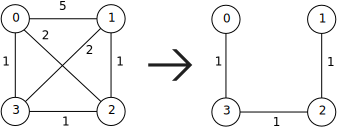
\includegraphics[width=0.75\textwidth,height=\textheight]{images/4.png}
\caption{Examples}
\end{figure}

\hypertarget{complete-trees}{%
\subsection{Complete Trees}\label{complete-trees}}

\begin{itemize}
\tightlist
\item
  Could only be missing nodes in their bottom row
\item
  Nodes in the bottom row are as far lest as possible
\end{itemize}

\begin{figure}
\centering
\includegraphics[width=0.5\textwidth,height=\textheight]{images/5.png}
\caption{Incomplete Trees}
\end{figure}

\begin{figure}
\centering
\includegraphics[width=0.5\textwidth,height=\textheight]{images/6.png}
\caption{Complete Trees}
\end{figure}

\hypertarget{trees-and-heaps-in-arrays}{%
\subsection{Trees and Heaps in Arrays}\label{trees-and-heaps-in-arrays}}

\begin{figure}
\centering
\includegraphics[width=0.5\textwidth,height=\textheight]{images/6.png}
\caption{A complete binary tree and its array representation}
\end{figure}

\begin{itemize}
\tightlist
\item
  The root is at index 1
\item
  Binary tree

  \begin{itemize}
  \tightlist
  \item
    \passthrough{\lstinline!left(i) = 2 * i!}
  \item
    \passthrough{\lstinline!right(i) = 2 * i + 1!}
  \item
    \passthrough{\lstinline!parent(i) = i / 2!}
  \end{itemize}
\end{itemize}

\hypertarget{road-map}{%
\subsection{Road Map}\label{road-map}}

\begin{itemize}
\tightlist
\item
  Priority queue

  \begin{itemize}
  \tightlist
  \item
    \passthrough{\lstinline!insert(T t)!},
    \passthrough{\lstinline!findMin()!},
    \passthrough{\lstinline!deleteMin()!}
  \end{itemize}
\item
  Heap

  \begin{itemize}
  \tightlist
  \item
    Complete binary tree
  \item
    Heap order

    \begin{itemize}
    \tightlist
    \item
      Min heap
    \item
      Max heap
    \end{itemize}
  \item
    Operations and complexity

    \begin{itemize}
    \tightlist
    \item
      Insert: percolate up
    \item
      Delete: percolate down
    \end{itemize}
  \end{itemize}
\item
  Heap sort
\end{itemize}

\hypertarget{priority-queue-operations-with-binary-heaps}{%
\subsection{Priority Queue Operations with Binary
Heaps}\label{priority-queue-operations-with-binary-heaps}}

\begin{itemize}
\tightlist
\item
  Use an internal \passthrough{\lstinline!T array[]!} for queue contents

  \begin{itemize}
  \tightlist
  \item
    Maintain min-heap order in array
  \item
    Make sure it is always a complete tree
  \end{itemize}
\item
  \passthrough{\lstinline!T findMin()!}

  \begin{itemize}
  \tightlist
  \item
    \passthrough{\lstinline!return array[root()];!}
  \end{itemize}
\item
  \passthrough{\lstinline!insert(T t, int p)!}

  \begin{itemize}
  \tightlist
  \item
    Insert at the end of the array, increment size

    \begin{itemize}
    \tightlist
    \item
      Might violate the min-heap order property
    \end{itemize}
  \item
    Fix by swimming the new element up (percolate up)
  \end{itemize}
\item
  \passthrough{\lstinline!deleteMin()!}

  \begin{itemize}
  \tightlist
  \item
    Simply removing the root will leave a hole
  \item
    We can swap the last value and the root to fill the hole

    \begin{itemize}
    \tightlist
    \item
      \passthrough{\lstinline!null!} out the last value (which prevents
      loitering)
    \item
      Decrement the size
    \item
      The new root \emph{might} not be minimal
    \end{itemize}
  \item
    Percolate the new root value down the tree
  \end{itemize}
\item
  Max heap follows the same ideas
\end{itemize}

\hypertarget{binary-heap-demo}{%
\subsection{Binary Heap Demo}\label{binary-heap-demo}}

\begin{itemize}
\tightlist
\item
  Starting from a min-heap like Example 2

  \begin{itemize}
  \tightlist
  \item
    Insert 50, 18, and 10
  \item
    \passthrough{\lstinline!deleteMin()!}
  \end{itemize}
\item
  Starting form an empty max-heap

  \begin{itemize}
  \tightlist
  \item
    Insert 2, 3, 5, 3, and 9
  \item
    \passthrough{\lstinline!deleteMax()!} five times
  \end{itemize}
\end{itemize}

\hypertarget{operation-details}{%
\subsection{Operation Details}\label{operation-details}}

\begin{itemize}
\tightlist
\item
  Basic questions

  \begin{itemize}
  \tightlist
  \item
    With whom do we compare or swap?
  \item
    When do we stop moving?
  \end{itemize}
\item
  Percolate up (bubble up)

  \begin{itemize}
  \tightlist
  \item
    Compare / swap with the parent
  \item
    Halting condition: when we reach the top (the root) or no longer
    violate the heap order
  \end{itemize}
\item
  Percolate down (sink down)

  \begin{itemize}
  \tightlist
  \item
    Compare / swap with a child
  \item
    Halting condition: when we reach the bottom (a leaf) or no longer
    violate the heap order
  \end{itemize}
\end{itemize}

\hypertarget{weiss-code-example}{%
\subsection{Weiss Code Example}\label{weiss-code-example}}

\begin{lstlisting}[language=Java]
/**
 * Removes the smallest item in the priority queue.
 * @return the smallest item.
 * @throws NoSuchElementException if empty.
 */
public T remove() {
  T minItem = element();
  // Move the tail element to the root
  array[1] = array[currentSize--];
  // Sink the new root down to fix the heap order
  percolateDown(1);
}

 /**
  * Internal method to percolate down in the heap.
  * @param hole the index at which to percolate begins.
  */
private void percolateDown(int hole) {
  int child;
  T tmp = array[hole];
  // Decide which child to compare/swap
  for (; hole * 2 <= currentSize; hole = child) {
    child = hole * 2;
    if (child != currentSize && compare(array[child+1], array[child]) < 0) {
      child++;
    }
    // Keep swapping with children until parent-child comparison result is 
    // satisfactory, or the bottom is reached
    if (compare(array[child], tmp) < 0) {
      array[hole] = array[child];
    } else {
      break;
    }
    array[hole] = tmp;
  }
}
\end{lstlisting}

\hypertarget{complexity-analysis}{%
\subsection{Complexity Analysis}\label{complexity-analysis}}

\begin{itemize}
\tightlist
\item
  \passthrough{\lstinline!findMin()!} is clearly \(O(1)\)
\item
  What about \passthrough{\lstinline!insert(T t)!} and
  \passthrough{\lstinline!deleteMin()!}?

  \begin{itemize}
  \tightlist
  \item
    Percolation does most of the work
  \item
    Worst case: \(O(\)height\()\)

    \begin{itemize}
    \tightlist
    \item
      Complete binary tree: \(O(\log(n))\)
    \end{itemize}
  \end{itemize}
\item
  Note: no \passthrough{\lstinline!get(T t)!} or
  \passthrough{\lstinline!remove(T t)!}
\end{itemize}

\hypertarget{priority-queues-comparison}{%
\subsection{Priority Queues
Comparison}\label{priority-queues-comparison}}

\begin{longtable}[]{ccccc}
\toprule
Data Structure & \passthrough{\lstinline!enqueue(T t)!} & peek\(^*\) &
dequeue\(^*\) & Notes\tabularnewline
\midrule
\endhead
Unsorted List & \(O(1)\) & \(O(n)\) & \(O(n)\) & best priority can be
any location\tabularnewline
Sorted Array & \(O(n)\) & \(O(1)\) & \(O(1)\) & best priority at high
index\tabularnewline
Sorted Linked List & \(O(n)\) & \(O(1)\) & \(O(1)\) & best at head or
tail\tabularnewline
Multiple Queues & \(O(1)\) & \(O(m)\) & \(O(m)\) & -\tabularnewline
Binary Search Tree & \(O(\)height\()\) & \(O(\)height\()\) &
\(O(\)height\()\) & min at left-most\tabularnewline
Binary Heap & \(O(\log(n))\) & \(O(1)\) & \(O(\log(n))\) & best priority
at root\tabularnewline
\bottomrule
\end{longtable}

\begin{itemize}
\tightlist
\item
  \(^*\): assuming best priority
\item
  \(n\): the number of items in a queue
\item
  \(m\): the number of priority levels
\end{itemize}

\end{document}
